\documentclass[11pt]{article}

\usepackage[margin=1in]{geometry}
\usepackage{amsmath}
\usepackage{amssymb}
\usepackage{hyperref}
\usepackage{microtype}
\usepackage{setspace}
\usepackage{xcolor}
\usepackage{booktabs}
\usepackage{caption}
\usepackage{float}
\usepackage{parskip}
\usepackage{tikz}
\usepackage{pgfplots}
\pgfplotsset{compat=1.18}
\usetikzlibrary{arrows.meta, positioning, shapes.geometric, calc, fit, backgrounds}

\definecolor{maleblue}{RGB}{70,130,180}
\definecolor{femalered}{RGB}{205,92,92}
\definecolor{teal}{RGB}{0,128,128}
\definecolor{boxgray}{RGB}{230,230,230}
\definecolor{boxblue}{RGB}{173,216,230}
\definecolor{boxgreen}{RGB}{144,238,144}
\definecolor{boxorange}{RGB}{255,218,185}

\hypersetup{
  colorlinks=true,
  linkcolor=teal,
  urlcolor=teal,
  citecolor=teal
}

\setlength{\parindent}{0pt}
\setlength{\parskip}{8pt}
\onehalfspacing

\title{\textbf{Mitigating Unfairness in Chest X-Ray Image Classifiers\\
Using Network Pruning and Adversarial Debiasing}}

\author{
  Riddhi Bhagwat \quad Courtney Ma \quad Maggie Lin \\[4pt]
  \small Final project for 6.7960, MIT
}

\date{}

\begin{document}

\maketitle
\tableofcontents
\newpage

% ─────────────────────────────────────────
\section{Introduction and Motivation}

With the increasing adoption of AI in healthcare, fairness in machine learning models has become a pressing concern, particularly in high-stakes applications like medical imaging. Models used for chest X-ray classification have achieved impressive accuracy in diagnosing diseases [1], yet their performance often varies across demographic groups. This disparity stems from biases embedded in both the training data and model architecture, leading to inequities in diagnostic outcomes. These observations raise critical questions: how can we mitigate such biases effectively? And what methods can ensure fairness without compromising model performance?

To tackle these questions, we first examine prior work in bias mitigation. A growing body of research highlights the limitations of single-method approaches. Adversarial debiasing, for instance, has been successfully applied to structured datasets to reduce gender bias in salary predictions (Yang et al., 2023) [4]. On the other hand, network pruning has proven effective at improving computational efficiency by removing redundant parameters, but its potential to address fairness remains underexplored (Marcinkevi\v{c}s et al., 2022) [6]. These techniques have been used independently, but few studies have combined their strengths to target fairness in medical imaging tasks.

One of the most challenging aspects of mitigating biases in medical imaging is addressing intersectional disparities, such as those arising from gender. [3] Demographic shortcuts---where models rely on superficial correlations rather than medically relevant features---pose unique challenges. As Tejani et al. (2024) [5] note, such shortcuts are particularly prevalent in medical imaging datasets due to underrepresentation and systemic biases. We hypothesize that the combination of adversarial debiasing and network pruning can offer a robust solution, with adversarial debiasing tackling the root causes of bias during training and network pruning refining the network post-training to further reduce bias-contributing units.

To assess the fairness of these methods, we turn to well-established metrics like false negative rate, equalized odds, and predictive parity, which evaluate the extent to which model predictions are consistent across demographic groups. These metrics are critical in ensuring that fairness improvements are measurable and actionable. For instance, the false negative rate metric requires that the rate of missed diagnoses (false negatives) is consistent across groups, while equalized odds ensures similar true negative and true positive rates across demographic groups. Predictive parity, meanwhile, focuses on the consistency of positive predictive values across groups. Together, these metrics provide a comprehensive framework for assessing and improving fairness.

In this project, we aim to bridge the gap between existing fairness methodologies and the unique challenges of medical imaging. By leveraging adversarial debiasing and network pruning in tandem, we hope to introduce a novel framework that not only mitigates biases but also offers insights into the interplay between computational efficiency and fairness in healthcare AI.


% ─────────────────────────────────────────
\section{Related Work}

\subsection{Adversarial Debiasing}

Adversarial debiasing is a widely used in-processing method that directly addresses systemic biases during training. This approach involves training two models simultaneously: a primary classifier and an adversary. The classifier aims to minimize prediction errors, while the adversary tries to predict protected attributes from the classifier's outputs. By learning to make predictions that are less informative about sensitive attributes, the classifier reduces bias in its outputs.

Yang et al. (2023) [4] demonstrated the effectiveness of adversarial debiasing in mitigating gender bias in salary prediction, showcasing its adaptability across domains. In healthcare, adversarial debiasing has been particularly effective in reducing disparities among demographic groups while maintaining diagnostic accuracy. However, the computational overhead introduced by this method remains a significant consideration, especially in resource-constrained settings.

\subsection{Network Pruning}

Network pruning, traditionally used for model compression and efficiency, has recently been adapted as a post-processing technique for bias mitigation. This method works by selectively removing neurons or parameters that contribute to biased predictions, thereby enhancing fairness while simultaneously improving computational efficiency.

Marcinkevi\v{c}s et al. (2022) [6] applied gradient-based pruning techniques to chest X-ray classifiers, achieving reductions in bias at intermediate network layers. Beyond fairness improvements, pruning optimized model size and inference speed, making it particularly suitable for scenarios with limited computational resources. While pruning is advantageous for its efficiency, its effectiveness in addressing complex biases is often limited when used as a standalone approach, highlighting its role as a complementary method.

\subsection{Fairness Metrics}

To evaluate the impact of adversarial debiasing and network pruning, fairness metrics provide a structured and quantitative framework. These metrics assess whether models treat all demographic groups equitably, allowing for systematic comparison of trade-offs between fairness, accuracy, and efficiency.

\subsubsection{False Negative Rate}

The false negative rate is the proportion of actual positive cases that are incorrectly predicted as negative. In the context of medical imaging, it captures cases where a disease is present but undetected by the model. This is critical in healthcare, where false negatives can delay treatment or result in missed diagnoses. The fairness goal is to ensure that the FNR is consistent across demographic groups:

\medskip
\noindent\hfill
False Negative Rate (FNR) $=\displaystyle\frac{\mathrm{FN}}{\mathrm{FN}+\mathrm{TP}}$
\hfill\null
\medskip

This metric aligns with clinical priorities, as it emphasizes equitable diagnostic outcomes. Reducing disparities in FNR ensures that under-diagnosed populations receive adequate attention, addressing systemic biases in healthcare delivery.

\subsubsection{Equalized Odds}

Equalized odds goes beyond false negative rate parity by ensuring that both true positive rates (TPR) and false positive rates (FPR) are consistent across groups. This ensures fairness not only in correct predictions but also in errors:

\medskip
\noindent\hfill
Equalized Odds Parity:\quad
$P(\hat{Y}=1 \mid A_a) = P(\hat{Y}=1 \mid A_b)\; \forall\, a,b \in A,\quad
P(\hat{Y}=1 \mid Y=1, A_a) = P(\hat{Y}=1 \mid Y=1, A_b)\; \forall\, a,b \in A,\; \forall\, y$
\hfill\null
\medskip

Yu and Zhai (2024) [2] argued that equalized odds is particularly important in healthcare, where unequal error rates could lead to disparities in treatment outcomes.

\subsubsection{Predictive Parity}

Predictive parity ensures that the positive predictive value (PPV) is consistent across groups, reflecting the likelihood of a positive prediction being correct. It is defined as:

\medskip
\noindent\hfill
Predictive Parity:\quad
$P(Y=1 \mid \hat{Y}=1, A=a) = P(Y=1 \mid \hat{Y}=1, A=b)\; \forall\, a,b \in A$
\hfill\null
\medskip

By leveraging these metrics, our project evaluates the trade-offs between fairness, accuracy, and computational efficiency. Adversarial debiasing, while computationally intensive, excels at bias mitigation, whereas network pruning complements it by offering computational efficiency with targeted fairness improvements. Together, these methods and metrics form a comprehensive approach to addressing bias in healthcare AI.


% ─────────────────────────────────────────
\section{Methodology}

For our experiments, we trained and validated the four different models on the same dataset. To evaluate these models, fairness metrics such as Equalized Odds (TPR and FPR parity), Predictive Parity (PPV), and False Negative Rate (FNR) parity were used to assess fairness between male and female groups. Additionally more general metrics like precision, recall, F1 scores, and loss were analyzed to ensure that performance stability was maintained.

\subsection{Data}

We used the CheXpert dataset [7], which contains 224,316 chest radiographs of 65,240 patients tested on 11 respiratory diseases each. For our training, we took a random sample of 1034 greyscale images and used a 80-20\% training-validation split. Each image is associated with demographic information, including sex and age, and has a positive or negative diagnosis for 11 diseases (Enlarged Cardiomediastinum, Cardiomegaly, Lung Opacity, Lung Lesion, Edema, Consolidation, Pneumonia, Atelectasis, Pneumothorax, Pleural Effusion, and Fracture). The gender distribution for both the training and validation dataset is shown in Figure~\ref{fig:gender_dist}. Both datasets are majority male, with 58.8\% of males in the training dataset and 54.7\% of males in the validation dataset.

% ── Figure 1: Gender Distribution ──
\begin{figure}[H]
\centering
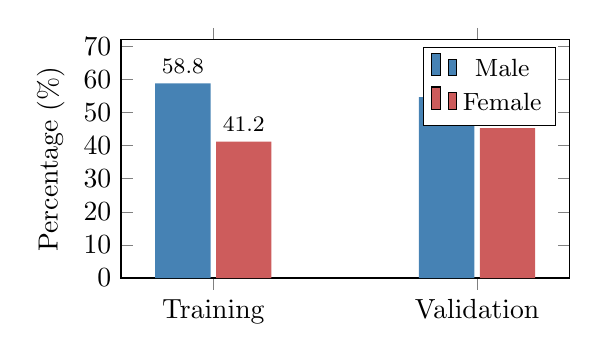
\begin{tikzpicture}
\begin{axis}[
  ybar,
  bar width = 20pt,
  width = 0.6\textwidth,
  height = 0.38\textwidth,
  symbolic x coords = {Training, Validation},
  xtick = data,
  ymin = 0, ymax = 72,
  ylabel = {Percentage (\%)},
  ytick = {0,10,20,30,40,50,60,70},
  legend style = {at={(0.97,0.97)}, anchor=north east, font=\small},
  nodes near coords,
  nodes near coords style = {font=\footnotesize},
  every axis plot/.append style = {draw=none},
  enlarge x limits = 0.35,
]
\addplot[fill=maleblue]  coordinates {(Training,58.8) (Validation,54.7)};
\addplot[fill=femalered] coordinates {(Training,41.2) (Validation,45.3)};
\legend{Male, Female}
\end{axis}
\end{tikzpicture}
\caption{Gender distribution for the training and validation datasets.}
\label{fig:gender_dist}
\end{figure}

\subsection{Model Architecture}

We implement four different CNN models total: a baseline model with no debiasing techniques, a model that utilizes adversarial debiasing, a model that utilizes pruning, and a model that utilizes both techniques. Each model takes in an X-Ray image and predicts a diagnosis for each of the 11 diseases. We utilize binary cross-entropy loss and an Adam optimizer for all models. All of the debiasing models adjust for bias in gender.

The baseline CNN model is a SimpleCNN with three convolutional layers. These layers are separated by ReLU nonlinearities followed by two fully connected layers. The input is the greyscale X-Ray image, while the output is predictions for each of the 11 diseases.

% ── Figure 2: SimpleCNN Architecture ──
\begin{figure}[H]
\centering
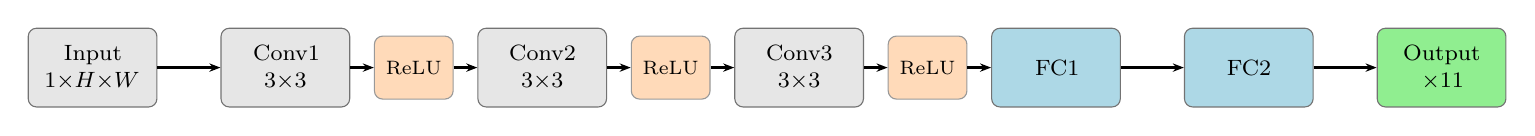
\begin{tikzpicture}[
  node distance = 5mm and 8mm,
  box/.style = {
    rectangle, rounded corners=3pt, draw=black!55,
    fill=boxgray, minimum width=15mm, minimum height=10mm,
    font=\footnotesize, align=center, text width=14mm
  },
  relu/.style = {
    rectangle, rounded corners=3pt, draw=black!40,
    fill=boxorange, minimum width=10mm, minimum height=8mm,
    font=\scriptsize, align=center
  },
  arr/.style = {-{Stealth[length=4pt]}, thick}
]
\node[box] (inp) {Input\\$1{\times}H{\times}W$};
\node[box,  right=of inp]  (c1)  {Conv1\\$3{\times}3$};
\node[relu, right=3mm of c1] (r1) {ReLU};
\node[box,  right=3mm of r1] (c2)  {Conv2\\$3{\times}3$};
\node[relu, right=3mm of c2] (r2) {ReLU};
\node[box,  right=3mm of r2] (c3)  {Conv3\\$3{\times}3$};
\node[relu, right=3mm of c3] (r3) {ReLU};
\node[box,  right=3mm of r3, fill=boxblue]  (fc1) {FC1};
\node[box,  right=of fc1,    fill=boxblue]  (fc2) {FC2};
\node[box,  right=of fc2,    fill=boxgreen] (out) {Output\\${\times}11$};
\draw[arr] (inp)--(c1); \draw[arr] (c1)--(r1); \draw[arr] (r1)--(c2);
\draw[arr] (c2)--(r2);  \draw[arr] (r2)--(c3); \draw[arr] (c3)--(r3);
\draw[arr] (r3)--(fc1); \draw[arr] (fc1)--(fc2); \draw[arr] (fc2)--(out);
\end{tikzpicture}
\caption{SimpleCNN baseline architecture.}
\label{fig:simplecnn}
\end{figure}

For the adversarial debiasing pipeline, we trained a Generative Adversarial Network (GAN) to mitigate gender bias. We built on the SimpleCNN baseline model and used a gradient reversal layer and two separate prediction branches: one for disease prediction and one for the sensitive gender attribute.

% ── Figure 3: Adversarial Debiasing Pipeline ──
\begin{figure}[H]
\centering
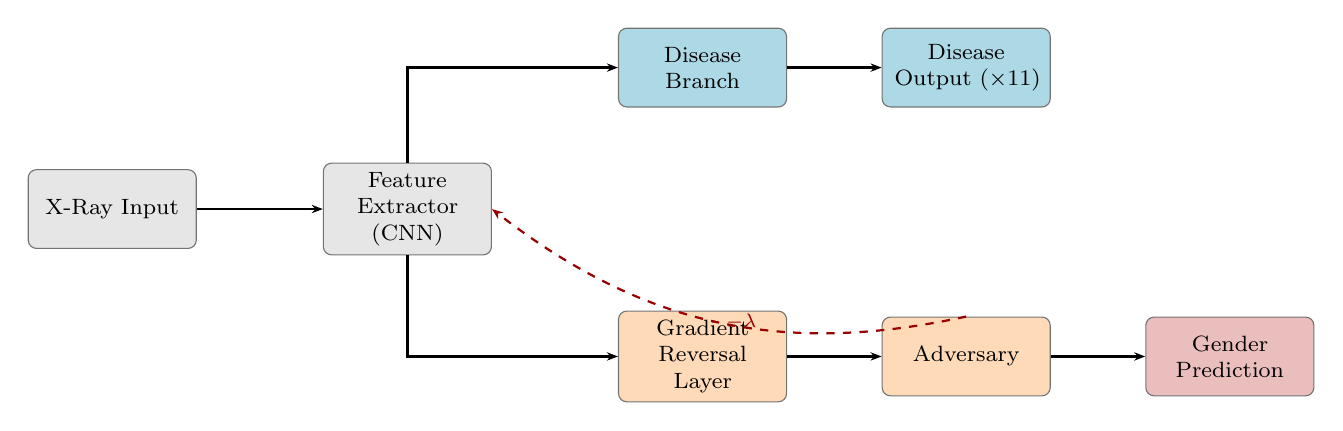
\begin{tikzpicture}[
  node distance = 7mm and 14mm,
  box/.style = {
    rectangle, rounded corners=3pt, draw=black!55,
    minimum width=20mm, minimum height=10mm,
    font=\footnotesize, align=center, text width=19mm
  },
  arr/.style = {-{Stealth[length=4pt]}, thick}
]
\node[box, fill=boxgray]   (inp)  {X-Ray Input};
\node[box, fill=boxgray,   right=16mm of inp]  (feat) {Feature\\Extractor\\(CNN)};
\node[box, fill=boxblue,   above right=7mm and 16mm of feat] (db)  {Disease\\Branch};
\node[box, fill=boxorange, below right=7mm and 16mm of feat] (grl) {Gradient\\Reversal Layer};
\node[box, fill=boxblue,   right=12mm of db]   (dout) {Disease Output (${\times}11$)};
\node[box, fill=boxorange, right=12mm of grl]  (adv)  {Adversary};
\node[box, fill=femalered!40, right=12mm of adv] (gout) {Gender\\Prediction};
\draw[arr] (inp)--(feat);
\draw[arr] (feat) |- (db);
\draw[arr] (feat) |- (grl);
\draw[arr] (db)--(dout);
\draw[arr] (grl)--(adv);
\draw[arr] (adv)--(gout);
\draw[arr, dashed, red!60!black, bend left=25]
  (adv.north) to node[right, font=\scriptsize]{$-\lambda$} (feat.east);
\end{tikzpicture}
\caption{Adversarial debiasing pipeline with gradient reversal layer and two prediction branches.}
\label{fig:adversarial}
\end{figure}

For the pruning only debiasing model, we identified which layer's hyperparameters contained the most amount of bias and minimized the bias from that layer by pruning its weights. We separately pruned 50\% of the weights for each convolutional layer from the baseline model, and calculated fairness metrics for each. Then, we compared the debiasing performance for pruning each layer, and selected the model with the least amount of bias. Figure~\ref{fig:pruning} shows the process of pruning convolutional layer 2, the most biased layer in the model. After pruning the biased weights in the layer (highlighted in red), the resulting model has less bias overall.

% ── Figure 4: Pruning Diagram ──
\begin{figure}[H]
\centering
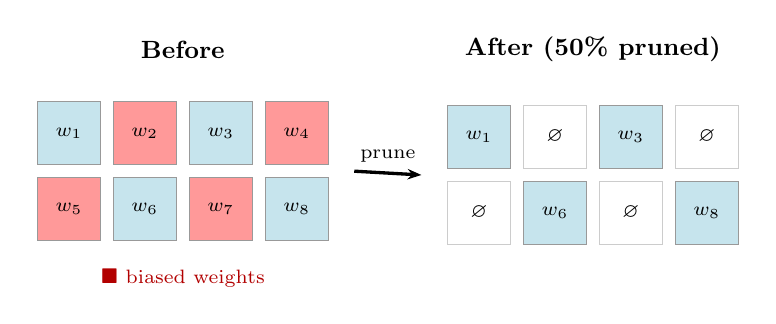
\begin{tikzpicture}[
  w/.style={rectangle, draw=black!40, minimum width=8mm, minimum height=8mm,
            font=\scriptsize, align=center},
  arr/.style={-{Stealth[length=5pt]}, very thick}
]
\node[font=\small\bfseries] (bl) {Before};
\matrix[below=3mm of bl, row sep=1.5mm, column sep=1.5mm, nodes={w}] (Wb) {
  \node[fill=boxblue!70]{$w_1$}; & \node[fill=red!40]{$w_2$}; &
  \node[fill=boxblue!70]{$w_3$}; & \node[fill=red!40]{$w_4$}; \\
  \node[fill=red!40]{$w_5$}; & \node[fill=boxblue!70]{$w_6$}; &
  \node[fill=red!40]{$w_7$}; & \node[fill=boxblue!70]{$w_8$}; \\
};
\node[font=\scriptsize, red!70!black, below=1mm of Wb]
  {{\color{red!70!black}$\blacksquare$} biased weights};

\node[font=\small\bfseries, right=28mm of bl] (al) {After (50\% pruned)};
\matrix[below=3mm of al, row sep=1.5mm, column sep=1.5mm, nodes={w}] (Wa) {
  \node[fill=boxblue!70]{$w_1$}; & \node[fill=white,draw=black!20]{$\varnothing$}; &
  \node[fill=boxblue!70]{$w_3$}; & \node[fill=white,draw=black!20]{$\varnothing$}; \\
  \node[fill=white,draw=black!20]{$\varnothing$}; & \node[fill=boxblue!70]{$w_6$}; &
  \node[fill=white,draw=black!20]{$\varnothing$}; & \node[fill=boxblue!70]{$w_8$}; \\
};

\draw[arr] ($(Wb.east)+(2mm,0)$) -- ($(Wa.west)+(-2mm,0)$)
  node[midway, above, font=\scriptsize]{prune};
\end{tikzpicture}
\caption{Pruning process for convolutional layer 2. Biased weights (red) are removed; the resulting model has less bias overall.}
\label{fig:pruning}
\end{figure}

Similarly, for the combined adversarial debiasing and pruning model, we use the adversarial debiasing framework and apply network pruning to the three convolutional layers in the model.


% ─────────────────────────────────────────
\section{Results}

We calculated our chosen fairness metrics for all four models. Our results are shown in Table~\ref{tab:results}.

% ── Table (replacing Figure 5) ──
\begin{table}[H]
\centering
\caption{Fairness metric gaps (male $-$ female) across all four models.
Cells marked `---' were not reported in the text.
\textbf{Please fill in any missing values from your original results.}}
\label{tab:results}
\renewcommand{\arraystretch}{1.3}
\begin{tabular}{lcccc}
\toprule
\textbf{Model} & \textbf{EO: TPR Gap} & \textbf{EO: FPR Gap} & \textbf{PP Gap} & \textbf{FNR Gap} \\
\midrule
Baseline                          & 0.0885 & 0.0112 & ---    & --- \\
Adversarial Debiasing Only        & 0.1043 & 0.0100 & ---    & --- \\
Pruning Only (conv2, 50\%)        & 0.0257 & ---    & ---    & --- \\
Combined (Adv.\ + Pruning conv2)  & 0.0280 & ${\sim}$0.01 & 0.0035 & --- \\
\bottomrule
\end{tabular}
\end{table}

\subsection{Baseline Model (No Debiasing)}

The SimpleCNN model, trained with no debiasing techniques, served as the baseline for fairness evaluation. It exhibited significant gender disparities in training and validation with female samples consistently underperforming compared to male samples across all metrics. Alongside the disparities in precision, recall, and F1 scores, the control model demonstrated significant imbalances in key fairness metrics, which further highlight the inherent biases in the dataset and model. The metrics shown in Table~\ref{tab:results} provide a deeper look into these disparities, where there is a large disparity between the male and female fairness metrics.

While the training and validation losses converged smoothly, the fairness metrics showed substantial imbalances, highlighting the limitations of conventional training without targeted debiasing. For example, equalized odds (True Positive Rate), males had a higher TPR compared to females, with a 0.885 difference.

\subsection{Adversarial Debiasing Only Model}

The model trained with adversarial debiasing showed improvements in some disparities compared to the baseline model, but on the whole seemed to exhibit increased discrepancies in true positive rates and predictive parity. Specifically, while the false positive rate decreased from 0.0112 to 0.01 compared to baseline, the gap between male and female true positive rates increased from 0.0885 to 0.1043 (8.85\% to 10.43\%).

\subsection{Pruning Only Model}

Pruning was applied to each convolutional layer at 50\% to assess its impact on gender bias and fairness metrics. After evaluating the results for convolutional layers 1, 2, and 3, we found that pruning convolutional layer 2 was the most effective in reducing fairness gaps, particularly in terms of True Positive Rate (TPR), where the gender gap decreased significantly. This suggests that mid-level features play a critical role in improving fairness without drastically sacrificing performance.

Pruning convolutional layer 3 also showed some improvements, particularly in False Positive Rate (FPR), but the TPR and Predictive Parity (PPV) gaps remained relatively wide. This suggests that deeper layers may capture more complex, abstract features that are harder to balance for fairness without a more sophisticated debiasing strategy.

On the other hand, pruning convolutional layer 1 (the shallowest layer) led to only minor reductions in fairness gaps, suggesting that low-level features may have a less significant impact on bias compared to mid-level or deep features. These results imply that a more targeted pruning strategy, particularly focusing on mid-level layers like convolution layer 2, could offer the best trade-off between fairness and model performance.

Therefore, we focus on the results for convolutional layer 2 in the following analysis, alongside the relevant fairness metrics.

\subsection{Pruning and Adversarial Debiasing Combined Model}

The integration of pruning with adversarial debiasing amplified fairness improvements, especially in conv2. The difference between female predictive parity and male predictive parity was reduced significantly to only 0.0035. The difference in true positive rates reached a point similar to when we used just pruning, with an approximate difference of 0.028. The gap in false positive rates between males and females was also at similar levels as the baseline model and the adversarial debiasing model without pruning (${\sim}$ 0.01). All of these metrics showed increased predictive power in reducing bias and the predictive parity results ensure that the precision rates for the disease subgroups are similar across subgroups.


% ─────────────────────────────────────────
\section{Discussion}

\subsection{Adversarial Debiasing}

There was a 1.58\% increase in disparity, which while unexpected, suggests that there was some underlying bias amplification during the adversarial training process. This could potentially be attributed to the adversarial debiasing model overfitting to the majority group's features or failing to adequately capture nuanced patterns in the minority group's data. Another possibility for this discrepancy could be mode collapse, a phenomenon common in GAN setups. This occurs when the model converges to a narrow subset of feature representations, neglecting the diversity of patterns present in the data, which can lead the adversarial debiasing model to overfit to the majority group's features or failing to adequately capture nuanced patterns in the minority group's data. Further investigation into the choice of adversarial loss, representation learning capacity, regularization techniques, and methods to counter mode collapse, such as gradient penalty or diversity-promoting constraints, might help mitigate such unintended consequences and improve fairness across demographic groups.

\subsection{Pruning}

Pruning convolutional layer 2 at 50\% led to good improvements in gender fairness metrics compared to our control model, which had no debiasing methods. In particular, pruning reduced the Equalized Odds (TPR) gap from 0.0885 in the control model to 0.0257, indicating less disparity between male and female performance. Additionally, Predictive Parity improved by 0.0534, further balancing gender-specific precision and recall.

In contrast, the control model showed larger fairness gaps, with substantial differences in Equalized Odds (TPR) and False Negative Rate (FNR) Parity, favoring males. These results suggest that without debiasing methods, the model learned biased patterns during training, especially in prediction accuracy across genders.

Pruning layer 2, which targets mid-level features, proved more effective in reducing bias than pruning shallow or deep layers. This highlights that pruning at this layer can achieve a better balance between fairness and performance.

Overall, pruning can effectively reduce gender bias, though it doesn't fully eliminate disparities.

\subsection{Combining Adversarial Debiasing and Pruning}

Combining both approaches revealed underlying trends in the debiasing approaches and demonstrated synergistic improvement in fairness metrics, particularly achieving near-perfect predictive parity, with the disparity between male and female predictive parity reduced to just 0.0035. This highlights the combined model's ability to ensure equitable precision rates across demographic groups. The true positive rate gap aligns closely with results achieved using pruning alone, suggesting that the pruning approach contributed significantly to reducing the TPR disparities. The fact that the false positive rate gap remains consistent with the baseline and adversarial debiasing models may indicate that the combined approach involves some tradeoff between pushing pruning towards decreasing TPR disparities and FPR disparities. Based on the data and trends we found, we hypothesize that the pruned layer will play a significant role in reducing the disparities in either the TPR or FPR metric depending on which metric has the largest disparity in a model that only leverages one of the approaches. This balance between fairness improvements and stability across metrics underscores the potential of this combined approach for fairness-sensitive applications. However, further analysis of model complexity and generalization trade-offs will be needed to confirm further claims regarding the model's capabilities in large-scale settings.

The results underscore the critical role of mid-level feature layers, particularly convolutional layer 2, in mitigating gender bias. Pruning these layers alone was effective in reducing disparities without degrading overall performance. While applying an adversarial debiasing pipeline to the original CNN architecture did not perform as well due to the various potential causes discussed, the combination of these techniques demonstrated a significant ability to improve fairness metrics, achieving more balanced performance across male and female samples.

The control model, trained without any explicit debiasing techniques, highlighted the limitations of conventional training approaches. Despite stable convergence in training and validation losses, the control model retained substantial gender disparities across all layers, indicating that training stability alone is insufficient for addressing bias.

Pruning and adversarial debiasing exhibited a synergy when applied strategically, particularly in convolutional layer 2. However, their integration posed challenges in convolutional layer 1 and convolutional layer 3, where the nature of the feature representations limited the effectiveness of these techniques. These findings emphasize the importance of layer-specific strategies in achieving robust bias mitigation.


% ─────────────────────────────────────────
\section{Conclusion \& Future Work}

This study evaluated the effectiveness of pruning and adversarial debiasing, independently and in combination, in reducing gender bias in convolutional neural networks. While adversarial debiasing alone performed worse than the baseline model, pruning alone proved effective at targeting mid-level feature layers, particularly convolutional layer 2, where significant improvements in fairness metrics were observed. The addition of adversarial debiasing enhanced these effects, achieving near-parity in performance metrics for male and female samples.

The control model, trained without debiasing techniques, demonstrated stable convergence but retained substantial gender disparities, emphasizing the necessity of targeted debiasing methods. While the combined approach of pruning and adversarial debiasing proved effective in mid-level layers, challenges in shallow and deep layers highlight the need for layer-specific strategies.

While our results did not exhibit the levels of high precision that we would have expected out of CNN training on CheXPert data, we hypothesize that incorporating more training data, including more convolutional layers, and training for longer time should be able to scale the accuracy and precision of all 4 approaches (including the control pipeline). Our current results show that the disparities were reduced with each added debiasing method. Pruning and adversarial debiasing alone both performed better than the control in terms of equalizing precision for females and males, and implementing adversarial debiasing with a pruned layer performed even better than both of them separately on this metric. With a larger scale of training data to prevent overfitting, increased complexity in model architecture to learn more nuanced trends, and more compute resources for fine-tuning the adversarial network, we expect these metrics to scale up and the marginal gaps between female and male predictions to become even more minute while overall precision is strengthened.

Future research should explore dynamic pruning strategies informed by adversarial gradients, refine loss functions for better compatibility between pruning and adversarial objectives, and investigate alternative approaches for addressing biases in shallow and deep layers. Further, with access to more resources, future studies can also leverage more compelx baseline model architectures, such as the ResNet-50, which may improve performance and amplify the effects of both debiasing techniques. By tailoring techniques to layer-specific characteristics, we can achieve greater fairness without sacrificing model performance.


% ─────────────────────────────────────────
\section*{References}

\noindent
[1] Geric, C et al. ``The rise of artificial intelligence reading of chest X-rays for enhanced TB diagnosis and elimination.'' \textit{The international journal of tuberculosis and lung disease} vol.\ 27,5 (2023): 367--372. doi:10.5588/ijtld.22.0687.

\bigskip\noindent
[2] Yu, Lanyi, and Xiaomei Zhai. ``Use of Artificial Intelligence to Address Health Disparities in Low- and Middle-Income Countries: A Thematic Analysis of Ethical Issues.'' \textit{Public Health}, vol.\ 234, 2024, pp.\ 77--83, doi:10.1016/j.puhe.2024.05.029.

\bigskip\noindent
[3] Yang, Yuzhe, et al. ``The Limits of Fair Medical Imaging AI in Real-World Generalization.'' \textit{Nature Medicine}, vol.\ 30, no.\ 10, 2024, pp.\ 2838--2848. doi:10.1038/s41591-024-03113-4.

\bigskip\noindent
[4] Yang, J., et al. ``An Adversarial Training Framework for Mitigating Algorithmic Biases in Clinical Machine Learning.'' \textit{NPJ Digital Medicine}, vol.\ 6, 2023, p.\ 55. \url{https://doi.org/10.1038/s41746-023-00805-y}.

\bigskip\noindent
[5] Tejani, Ali S., et al. ``Understanding and Mitigating Bias in Imaging Artificial Intelligence.'' \textit{RadioGraphics}, vol.\ 44, no.\ 5, 2024, p.\ e230067. doi:10.1148/rg.230067.

\bigskip\noindent
[6] Marcinkevi\v{c}s, Ri\v{c}ards, Ece Ozkan, and Julia E.\ Vogt. ``Debiasing Deep Chest X-Ray Classifiers Using Intra- and Post-Processing Methods.'' arXiv, 2022, \url{https://arxiv.org/abs/2208.00781}.

\bigskip\noindent
[7] Yi, P.\ H., Kim, T.\ K., Siegel, E., \& Yahyavi-Firouz-Abadi, N.\ (2022). Demographic reporting in publicly available chest radiograph data sets: Opportunities for mitigating sex and racial disparities in deep learning models. \textit{Journal of the American College of Radiology}, 19(1, Part B), 192--200.

\end{document}
